\section{Forward Plan}

As of writing this there has been a single publication from this project (outlined in \cref{sec:method-technosignature-searches}) with numerous other in preparation. \Cref{fig:gannt_chart} outlines the estimated timeline for the completion of all outlined projects.

\begin{figure}[h]
    \centering
    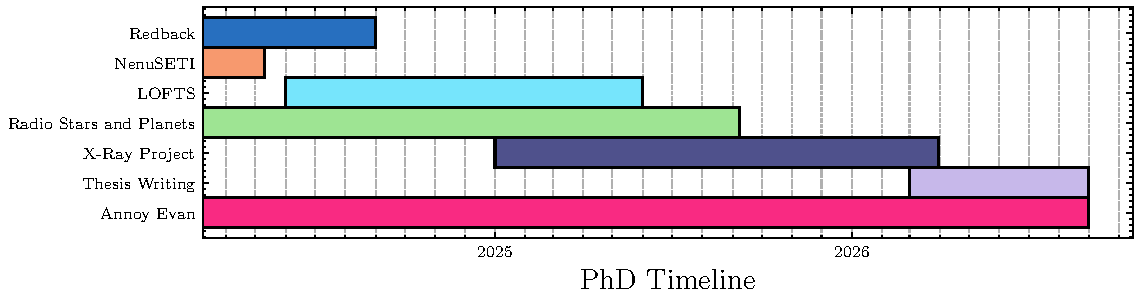
\includegraphics[width=0.95\textwidth]{figs/PhD_gannt_chart.pdf}
    \caption{Estimated timeline for compleltion of these projects which was covered in . Each increment on the grid is equivalent to 1 month.}
    \label{fig:gannt_chart}
\end{figure}

\textbf{NenuSETI} has had 80\% of the analysis complete. This paper is currently being drafted and once some system adminstration with the BL backend in Nancay is complete, the paper will be swiftly submitted no latter than the end of April 2024. \\ 

\textbf{Redback Pulsar Search} has full analysis pipelines written and deployed on the OzStar supercomputing cluster in Swinburne and REALTA backend in Birr. As of writing, all data from J2059 has been processed with expanded trials commencing to try and find the pulsar. Processing on J2054 is 50\% complete but temporarily halted due to some bottlenecking on the backend. Expected publication date of either a pulsar detection or non-detection is expected by the end August 2024. \\

\textbf{LOFTS} as previously discussed in X, the observation campaign is expected to commence following the roll out of LOFAR 2.0 upgrades to the core stations in the Netherlands. This is expected to happen in the early Summer months of 2024. This will cause all remote stations to be given 100\% of observing time, thus the large amount of observation time for LOFTS can be accomidated. \\ Automated pipelines to handle the data are written and tested on operational backends. Deployment of BL backend to the Chilboltan station is expected to be completed in the coming months. \\ 

\textbf{Radio Stars and Planets} \\ 

\textbf{X-ray Project}

\section{Conclusion}